% TEMPLATE for Usenix papers, specifically to meet requirements of
%  USENIX '05
% originally a template for producing IEEE-format articles using LaTeX.
%   written by Matthew Ward, CS Department, Worcester Polytechnic Institute.
% adapted by David Beazley for his excellent SWIG paper in Proceedings,
%   Tcl 96
% turned into a smartass generic template by De Clarke, with thanks to
%   both the above pioneers
% use at your own risk.  Complaints to /dev/null.
% make it two column with no page numbering, default is 10 point

% Munged by Fred Douglis <douglis@research.att.com> 10/97 to separate
% the .sty file from the LaTeX source template, so that people can
% more easily include the .sty file into an existing document.  Also
% changed to more closely follow the style guidelines as represented
% by the Word sample file. 

% Note that since 2010, USENIX does not require endnotes. If you want
% foot of page notes, don't include the endnotes package in the 
% usepackage command, below.

% This version uses the latex2e styles, not the very ancient 2.09 stuff.
\documentclass[10pt]{sig-alternate-05-2015}
\usepackage[T1]{fontenc}
\usepackage{times}  
\usepackage{epsfig}
\usepackage{afterpage}
\usepackage{tabularx}
\usepackage{graphicx}
\usepackage{balance}
\usepackage{color}
\usepackage{xcolor}
\usepackage{xspace}
\usepackage{thumbpdf}
\usepackage{listings}
\usepackage{verbatim}
\usepackage{color}
\usepackage[hidelinks]{hyperref}
\definecolor{darkred}{rgb}{0.7,0,0}
\definecolor{darkgreen}{rgb}{0,0.5,0}
\hypersetup{colorlinks=true,
        linkcolor=darkred,
        citecolor=darkgreen}
\usepackage{booktabs}
\usepackage{colortbl}
\usepackage[inline]{aplcomments}
\usepackage{inconsolata}
\usepackage{paralist}
\usepackage{xspace}
\usepackage{listings}
\usepackage{breakurl}
\usepackage{inconsolata}
\usepackage{longtable}
\usepackage{placeins}
\usepackage{caption, subcaption}
\usepackage{pbox}
\usepackage{pifont}% http://ctan.org/pkg/pifont
\usepackage{tablefootnote}
\usepackage{siunitx}
\newcommand{\cmark}{\ding{51}}%
\newcommand{\xmark}{\ding{55}}%
\lstset{
  basicstyle=\ttfamily,
  mathescape
}

\newcommenter{ak}{1.0,1.0,0.3}
\newcommenter{ac}{0.4,1.0,1.0}
\newcommand{\pktlanguage}{Domino\xspace}
\newcommand{\absmachine}{Banzai\xspace}
\newcommand{\tester}{Jayhawk\xspace}

\lstdefinestyle{customc}{
 belowcaptionskip=1\baselineskip,
 breaklines=true,
 xleftmargin=20pt,
 language=C,
 frame=L,
 escapeinside={@}{@},
 showstringspaces=false,
 basicstyle=\small\ttfamily,
 keywordstyle=\bfseries\color{green!40!black},
 commentstyle=\itshape\color{purple!40!black},
 %identifierstyle=\color{blue},
 stringstyle=\color{orange},
 directivestyle=\color{brown},
 numbers=left, numberstyle=\tiny\color{gray}
}


\lstdefinestyle{customctable}{
 aboveskip=-\medskipamount,
 belowskip=-\medskipamount,
 language=C,
 escapeinside={@}{@},
 showstringspaces=false,
 basicstyle=\scriptsize\ttfamily,
 keywordstyle=\bfseries\color{green!40!black},
 commentstyle=\itshape\color{purple!40!black},
 %identifierstyle=\color{blue},
 stringstyle=\color{orange},
 directivestyle=\color{brown},
}

\def\compactify{\itemsep=0pt \topsep=0pt \partopsep=0pt \parsep=0pt}
\let\latexusecounter=\usecounter
\newenvironment{CompactItemize}
  {\def\usecounter{\compactify\latexusecounter}
   \begin{itemize}}
  {\end{itemize}\let\usecounter=\latexusecounter}
\newenvironment{CompactEnumerate}
  {\def\usecounter{\compactify\latexusecounter}
   \begin{enumerate}}
  {\end{enumerate}\let\usecounter=\latexusecounter}


  \usepackage{hyperref}
  \def\UrlBreaks{\do\/\do-}
  \setlength{\parskip}{0pt}

%\newcommand{\MA}[1]{{({\color{blue}MA: #1})}}
\newcommand{\MA}[1]{}
\newcommand{\hb}[1]{}

\begin{document}


\sloppypar
\setcopyright{acmlicensed}
\conferenceinfo{SIGCOMM'16,}{August 22--26, 2016, Florianopolis, Brazil}

\acmPrice{\$15.00}

%TODO: doi
%don't want date printed
\date{}

%make title bold and 14 pt font (Latex default is non-bold, 16 pt)
\title{Packet Transactions: High-Level Programming for Line-Rate Switches}
\author{
\alignauthor \fontsize{10.7}{9.9}\selectfont Anirudh Sivaraman\textsuperscript{\P}, Mihai Budiu\textsuperscript{\S}\thanks{Work done when employed at Barefoot Networks.}, Alvin Cheung\textsuperscript{\ddag}, Changhoon Kim\textsuperscript{\dag}, Steve Licking\textsuperscript{\dag}, \fontsize{10.7}{9.9}\selectfont George Varghese\textsuperscript{++}, Mohammad Alizadeh\textsuperscript{\P}, Hari Balakrishnan\textsuperscript{\P}, Nick McKeown\textsuperscript{+}\\
\affaddr \fontsize{9.6}{9.9}\selectfont \textsuperscript{\P}MIT CSAIL, \textsuperscript{\S}VMWare Research, \textsuperscript{\ddag}University of Washington, \textsuperscript{\dag}Barefoot Networks, \textsuperscript{++}Microsoft Research, \textsuperscript{+}Stanford University
}
% copy the following lines to add more authors
% \and
% {\rm Name}\\
%Name Institution
%} % end author

\maketitle

% Use the following at camera-ready time to suppress page numbers.
% Comment it out when you first submit the paper for review.
%\thispagestyle{empty}
% 4. Start off each section with a "What's hard about this".
\section*{Abstract}

Data-plane algorithms encompass a wide-variety of packet processing
routines. Such algorithms are usually
implemented in hardware, whose inflexibility prohibits
experiments with new designs. While programmable switches have been
proposed as an alternative, they are often difficult to program due 
to limited language support. In this paper, we propose \pktlanguage, 
a new language for expressing data-plane algorithms on programmable
switches. \pktlanguage is a high-level, imperative language where 
developers express data-plane algorithms using packet functions with
transactional semantics. In this paper we describe our prototype compiler that
translates \pktlanguage programs into P4 scripts that can be implemented
in programmable switches, and our experience in using \pktlanguage to 
implement several data-plane algorithms. 


\begin{CCSXML}
<ccs2012>
<concept>
<concept_id>10003033.10003099.10003102</concept_id>
<concept_desc>Networks~Programmable networks</concept_desc>
<concept_significance>500</concept_significance>
</concept>
</ccs2012>
\end{CCSXML}

\ccsdesc[500]{Networks~Programmable networks}

\printccsdesc

\keywords{Programmable switches; stateful data-plane algorithms}

\section{Introduction}
\label{s:intro}

Network switches and routers in modern datacenters, enterprises, and
service provider networks are required to perform a variety of tasks
in addition to standard packet forwarding. The set of requirements for
routers has only been increasing with time as network operators have
sought to exercise greater control over performance and security, and
to support an evolving set of network protocols.

%TODO: Consider Alvin's point about global shared state
% being another feature of domino.
Performance and security may be improved using both data-plane and
control-plane mechanisms. This paper focuses on data-plane algorithms
for traffic management running in a switch. These algorithms process
every data packet, transforming the packet and often also some state
maintained in the switch.  Examples of such algorithms include
congestion control with switch feedback~\cite{xcp, rcp, pdq, dctcp},
active queue management~\cite{Floyd93,BLUE,pi,AVQ,REM,codel,pie},
network measurement~\cite{opensketch, bitmap_george, elephant_george,
  heavyhitters}, and load-balanced routing in the data
plane~\cite{conga}.

Because data-plane algorithms process every packet, an important
requirement is the ability to process packets at the line rate.  As a
result, these algorithms are typically implemented using dedicated
hardware. However, hardware designs are rigid and prevent
reconfigurability in the field making it difficult to implement and
deploy new algorithms without investing in new hardware---a
time-consuming and expensive proposition.

This rigidity affects vendors~\cite{cisco_nexus, dell_force10,
  arista_7050} building network switches with merchant-silicon
chips~\cite{trident, tomahawk, mellanox}, network operators deploying
switches~\cite{google,facebook,vl2}, and researchers developing new
switch algorithms~\cite{xcp, codel, d3, detail, pdq}.
%
%Today, the only way to implement a new data-plane algorithm at line rate
%is to build hardware for it.
To run data-plane algorithms after a switch has been built and
deployed, researchers and companies have attempted to build
programmable routers for many years, starting from efforts on active
networks~\cite{active-nets} to network processors~\cite{npu_survey} to
software routers~\cite{click,routebricks}. All these efforts have
compromised on speed to provide programmability, typically running an
order of magnitude (or worse) slower than hardware line
rates. Unfortunately, such a reduction in performance has meant that
these systems are rarely deployed in production networks, if at all.

Programmable switching chips~\cite{flexpipe, xpliant, rmt}, which are
competitive with state-of-the-art fixed-function
chipsets~\cite{trident, tomahawk, mellanox}, are a recent alternative.
These chips implement a few low-level hardware primitives that can be
configured by software into a processing
pipeline~\cite{xpliant_sdk,xpliant_sdk2,intel_sdk,rmt, P4}. This
approach is attractive because it does not compromise on data rates
and the area overhead is small.

%Programming these chips has
%become more user-friendly over time.  Initially, such chips were
%programmed using proprietary SDKs such as those from
%XPliant~\cite{xpliant_sdk, xpliant_sdk2} and
%Intel~\cite{intel_sdk}. Such SDKs closely resemble the underlying
%chipset, making them inconvenient for network programmers who are more
%familiar with a language like C.

P4~\cite{p4, p4spec} is a packet-processing language for switching
chips that raises the level of abstraction relative to these SDKs.
For instance, P4 allows the programmer to specify packet parsing and
processing without restricting the set of protocol formats or the set
of actions that can be executed when matching packet headers in a
match-action table. Many common data-plane tasks that require header
rewriting can now be expressed without naturally in P4, such as
handling new protocol formats, switching, forwarding, tunneling, and
access control~\cite{dc_p4}.

However, P4 today isn't suited to data-plane algorithms for congestion control,
load balancing, measurement and active queue management. These algorithms don't
rewrite headers, but instead manipulate internal switch state in a manner
unique to each algorithm.  For such data-plane algorithms, network programmers
would prefer the convenience of an imperative language such as C that directly
captures the algorithm's intent without shoehorning them into hardware
constructs such as a sequence of match-action tables like P4 requires them to.
Furthermore, this is predominantly how such data-plane algorithms are
implemented today in sofware routers~\cite{click, dpdk, routebricks}, network
processors~\cite{packetc, nova} and the Linux qdisc subsystem~\cite{qdisc} or
expressed as pseudocode when initially developed~\cite{red, csfq, codel_code,
avq, blue}.

This paper presents \pktlanguage, a new domain-specific language (DSL) for
data-plane algorithms.  \pktlanguage is an imperative language based on C that
allows programmers to express data-plane algorithms using {\em packet
transactions} (\S\ref{s:transactions}).  Packet transactions provide the
abstraction of a sequential block of code that runs to completion on each
packet before executing on the next packet. This is a convenient programming
model, because it allows the programmer to focus on the operations needed for
each packet without worrying about other packets that are concurrently being processed.

% Anirudh->Alvin: I don't like the phrase "to be executed".
% It sounds like a processor, and is a little wierd to me grammatically.
% Technically, we would say to binaries that execute on a family of abs. machines,
% but that would require explaining how we generate the binaries and again gives
% the impression of a processor.
% compiling to \absmachine is my fix to this, and is what we use in the proposal.
We have implemented a \pktlanguage compiler that compiles packet transactions
to a family of abstract machines called \absmachine~(\S\ref{s:absmachine}) (for
Protocol-Independent Switch Architecture). \absmachine generalizes the
Reconfigurable Match-Action Table~\cite{rmt} model and captures essential
features of line-rate programmable switches~\cite{rmt, xpliant, flexpipe}. In
addition, \absmachine introduces {\em atoms} to represent atomic computations
provided natively by a \absmachine machine, much like
load-link/store-conditional, and packed-multiply-and-add on x86 machines
today~\cite{x86_manual}.  Atoms provide hardware support for packet
transactions, similar to how an atomic test-and-set can implement an atomic
increment.

To evaluate \pktlanguage, we express data-plane algorithms~(\S\ref{s:eval})
such as RCP~\cite{rcp}, CoDel~\cite{codel}, heavy-hitter
detection~\cite{opensketch}, and CONGA~\cite{conga}, as packet transactions in
\pktlanguage. Expressing these algorithms involved a straightforward
translation of each algorithm's reference code to \pktlanguage syntax.  The
\pktlanguage compiler guarantees deterministic performance for these
algorithms: all packet transactions that compile run at line rate on a
\absmachine machine, or will be rejected by the compiler.  We use the
\pktlanguage compiler to determine if each algorithm can run at line rate on
several different \absmachine machines that differ in the atoms they provide
(Table~\ref{tab:algos}).

Overall, our results suggest that it is possible to have both a familiar
programming model, resembling DSLs for software routers and NPUs, and line-rate
performance---contrary to concerns raised in~\cite{p4} regarding the
unsuitability of expressive languages for line-rate packet processing.

\section{A Machine Model for Line-rate Switches}
\label{s:absmachine}
\begin{figure*}[!t]
  \includegraphics[width=\textwidth]{banzai.pdf}
  \caption{\absmachine models the ingress and egress pipelines of a
  programmable switch. Each atom corresponds to an action in a match-action
  table. Internally, an atom contains local state and a digital circuit that
  operates on this state. Figure~\ref{fig:atom} shows an atom in greater detail.}
  \label{fig:switch}
\end{figure*}

\absmachine is a machine model for programmable line-rate switches that serves
as the compiler target for \pktlanguage.  \absmachine is inspired by recent
programmable switch architectures such as Barefoot Networks' Tofino~\cite{tofino},
Intel's FlexPipe~\cite{flexpipe}, and Cavium's XPliant Packet
Architecture~\cite{xpliant}. \absmachine abstracts these architectures and
extends them with stateful processing units to implement data-plane algorithms.
These processing units, called {\em atoms}, model the set of atomic operations
that a hardware target can execute at line rate.

\subsection{Background: Programmable switches}
Packets arriving at a switch~(top half of Figure~\ref{fig:switch}) are parsed
by a programmable parser that turns packets into header fields. These header
fields are first processed by an ingress pipeline consisting of match-action
tables arranged in stages. Processing a packet at a stage may modify its header
fields, through match-action rules, as well as some persistent state at that
stage, e.g., packet counters. After the ingress pipeline, the packet is
queued. Once the scheduler dequeues the packet, it is processed by a
similar egress pipeline before it is transmitted.

To reduce chip area, there is only one ingress and one egress pipeline.  This
single pipeline is shared across all switch ports and handles aggregate traffic
belonging to all ports, at all packet sizes.  For instance, a 64-port switch
with a line rate of 10 Gbit/s per port and a minimum packet size of 64 bytes
needs to process around a billion packets per second, after accounting for
minimum inter-packet gaps~\cite{rmt}.  Equivalently, the pipeline runs at 1
GHz, and pipeline stages process a packet every clock cycle (1 ns).  We assume
one packet per clock cycle throughout the paper, and for concreteness, a
1 GHz clock frequency.

Having to process a packet every clock cycle in each stage greatly constrains
the operations that can be performed on each packet. In particular, any packet
operation that modifies state visible to the next packet {\em must} finish
execution in a single clock cycle (see \S\ref{ss:atoms} for details). Because
of this restriction, programmable switching chips provide a small set of
processing units or primitives for manipulating packets and state in a stage,
unlike software routers. These processing units determine the algorithms that
run on the switch at line rate.
%TODO: must finish within a clock cycle is a bit too strong, I think.

The challenge for us is to develop primitives that allow a broad range of
data-plane algorithms to be implemented, and to build a compiler to map a
user-friendly description of an algorithm to the primitives provided by a
switch.

\subsection{The \absmachine machine model}

\absmachine (the bottom half of Figure~\ref{fig:switch}) models
the ingress or egress switch pipeline.  It models the
computation within a match-action table in a stage (i.e., the action half of
the match-action table), but not how packets are matched (e.g., direct or
ternary). We discuss how to embed \absmachine in a standard match-action
pipeline in \S\ref{ss:guards}.  \absmachine also does not model packet parsing and assumes
that packets arriving to \absmachine are already parsed.

 Concretely, \absmachine is a feed-forward pipeline\footnote{It is hard to
physically route backward-flowing wires that would be required for feedback.}
consisting of a number of stages executing synchronously on every clock cycle.
Each stage processes one packet every clock cycle and hands it off to the next.
Unlike a CPU pipeline, which occasionally suffers from pipeline stalls,
\absmachine's pipeline is deterministic, never stalls, and always sustains line
rate. However, relative to a CPU pipeline, \absmachine is restricted in the
operations it supports (\S\ref{s:atomConstraints}).

\subsection{Atoms: \absmachine's processing units}
\label{ss:atoms}
 An {\em atom} is an atomic unit of packet processing supported natively by a
\absmachine machine, and the atoms within a \absmachine machine form its
instruction set. Each pipeline stage in \absmachine contains a vector of atoms.
Atoms in the vector modify mutually exclusive sections of the same packet
header in parallel in every clock cycle, and process a new packet header every
clock cycle.

In addition to packet headers, atoms may modify persistent state on the switch
to implement stateful data-plane algorithms. To support such algorithms at
line-rate, the atoms for a \absmachine machine need to be substantially richer
(Table~\ref{tab:templates}) than the simple RISC-like stateless instruction
sets for programmable switches today~\cite{rmt}. We explain why below.

Suppose we need to atomically increment a switch counter to count packets. One
approach is hardware support for three simple single-cycle operations:
\textit{read} the counter from memory in the first clock cycle, \textit{add}
one in the next, and \textit{write} it to memory in the third.  This approach,
however, does not provide atomicity. To see why, suppose packet $A$ increments
the counter from 0 to 1 by executing its read, add, and write at clock cycles
1, 2, and 3 respectively.  If packet $B$ issues its read at time 2, it will
increment the counter again from 0 to 1, when it should be incremented to 2.

Locks over the shared counter are a potential solution.  However, locking
causes packet $B$ to wait during packet $A$'s increment, and the switch no
longer sustains the line rate of one packet every clock cycle. CPUs employ
microarchitectural techniques such as operand forwarding to address this
problem, but CPUs still suffer the occasional pipeline stall, which prevents
line-rate performance from being achieved.

\absmachine provides an atomic increment operation at line rate with an {\em
atom} to read a counter, increment it, and write it back in a single stage within
one clock cycle. It uses the same approach of reading, modifying, and writing
back to implement other stateful atomic operations at line rate.

Unlike stateful atomic operations, stateless atomic operations are easier to
support with simple packet-field arithmetic.  Consider, for
instance, the operation {\tt pkt.f1 = pkt.f2 + pkt.f3 - pkt.f4}.  This
operation does not modify any persistent switch state and only accesses packet
fields. It can be implemented atomically by using two atoms: one atom to add
fields f2 and f3 in one pipeline stage, and another to subtract f4 from the
result in the next. An instruction set designer can provide {\em simple}
stateless instructions on pairs of packet fields alone, which can then be
composed into larger stateless operations, without designing atoms specifically
for each stateless operation.

\new{
\paragraph{Representing atoms}
An atom is represented by a body of sequential code that captures the atom's
behavior. It may also contain internal state local to the atom. An atom
completes execution of this entire body of code, modifying a packet and any
internal state before processing the next packet. The designer of a
programmable switch would develop these atoms, and expose them to a switch
compiler as the programmable switch's instruction set, e.g.,
Table~\ref{tab:templates}.
}
Using this representation, a switch counter that wraps around at a
value of 100 can be written as the atom:\footnote{We use {\tt p.x} to
  represent field {\tt x} within a packet {\tt p} and {\tt x} to
  represent a state variable {\tt x} that persists across packets.}
\begin{lstlisting}[style=customc, numbers=none, frame=none]
if (counter < 99)
  counter++;
else
  counter = 0;
\end{lstlisting}

Similarly, a stateless operation like setting a packet field to a constant
value can be written as the atom:
\begin{lstlisting}[style=customc, numbers=none, frame=none]
  p.field = value;
\end{lstlisting}

%TODO: Flip flopping between constraints and limits
\subsection{Constraints for line-rate operation}
\label{s:atomConstraints}

\new{
\textbf{Memory limits: } State in \absmachine is local to each atom.  It can
neither be shared by atoms within a stage, nor atoms across stages. This is
because building multi-ported memories accessible to multiple atoms is
technically challenging and consumes additional chip area. However, state can
be read into a packet header in one stage for subsequent use by a downstream
stage\footnote{Figure~\ref{fig:flowlet_pipeline} shows an example. {\tt
last\_time} is read into {\tt pkt.last\_time} in stage 2, for subsequent use by stage 3.}.  But, the \absmachine pipeline is
feed-forward, so state can only be carried forward, not backward.
}

\textbf{Computational limits:} Atoms need to execute atomically from one packet
to the next, so any state internal to the atom must be updated
before the next packet arrives.  Because packets may be separated by as little
as one clock cycle, we mandate that atom bodies finish execution within one
clock cycle, and constrain atom bodies to do so.

We constrain atom bodies by defining {\it atom templates}
(\S\ref{ss:code_gen}).  An atom template is a program with configurable
parameters that terminates within a clock cycle and specifies the atom's
behavior.  An example is an ALU with a restricted set of primitive operations
(Figure~\ref{fig:alu_diag}).

% Atom templates allow us to create
%and experiment with \absmachine machines with different atoms.

%As programmable
%switches evolve, we expect that atoms will evolve as well, but constrained by
%the clock-cycle requirement.

\begin{figure}[h]
  \begin{subfigure}{0.4\columnwidth}
  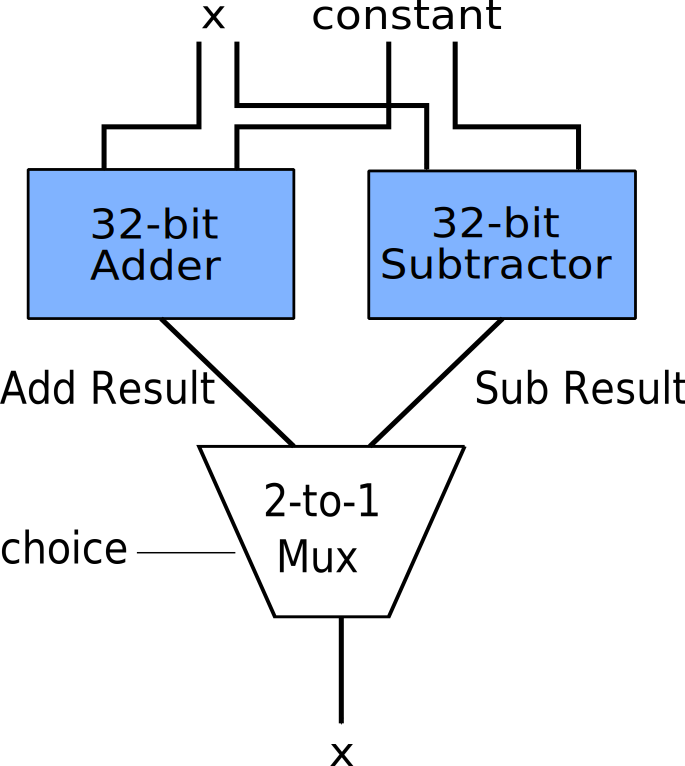
\includegraphics[width=\textwidth]{circuit.pdf}
  \caption{Circuit for the atom}
  \label{fig:alu_diag}
  \end{subfigure}
  \hspace{0.05\columnwidth}
  \begin{subfigure}{0.55\columnwidth}
  \begin{lstlisting}
  bit choice = ??;
  int constant = ??;
  if (choice) {
    x = x + constant;
  } else {
    x = x - constant;
  }
  \end{lstlisting}
  \caption{Atom template}
  %Each ``??(n)'' represents a hole that can be filled in with values in $[0, 2^n -1]$.}
  \label{fig:alu_in_sketch}
  \end{subfigure}
  \caption{An atom and its template. The atom above can add or subtract a constant from a state
  variable {\tt x} based on two configurable parameters, {\tt constant} and {\tt choice}.}
  \label{fig:atom}
\end{figure}

\textbf{Resource limits:} We also limit the number of atoms in each stage
(\textit{pipeline width}) and the number of stages in the pipeline
(\textit{pipeline depth}). This is similar to limits on the number of stages,
tables per stage, and memory per stage in programmable switch
architectures~\cite{lavanya_compiler}.

\subsection{What can \absmachine not do?}
\label{ss:limitations}

\absmachine is a good fit for data-plane algorithms that modify a small set of
packet headers and carry out small amounts of computation per packet.
Data-plane algorithms like deep packet inspection and WAN optimization require
a switch to parse and process the packet payload as well---effectively parsing
a large ``header'' consisting of each byte in the payload. This is challenging
at line rates of 1 GHz, and such algorithms are best left to CPUs~\cite{e2}.
Some algorithms require complex computations, but not on every packet, e.g., a
measurement algorithm that periodically scans a large table to perform garbage
collection.  \absmachine's atoms model small operations that occur on every
packet, and are unsuitable for such operations that span many clock cycles.

%TODO: Talk about how transactions can be composed.
% We 'll need to do this for the PIFO work as well.

\section{Packet transactions}
\label{s:transactions}

\begin{figure*}[!t]
\begin{minipage}{0.5\textwidth}
\begin{small}
\begin{lstlisting}[style=customc]
#define NUM_FLOWLETS    8000
#define THRESHOLD       5
#define NUM_HOPS        10

struct Packet {
  int sport;
  int dport;
  int new_hop;
  int arrival;
  int next_hop;
  int id; // array index
};

int last_time [NUM_FLOWLETS] = {0};
int saved_hop [NUM_FLOWLETS] = {0};

void flowlet(struct Packet pkt) {
  pkt.new_hop = hash3(pkt.sport,
                      pkt.dport,
                      pkt.arrival)
                % NUM_HOPS;

  pkt.id  = hash2(pkt.sport,
                  pkt.dport)
            % NUM_FLOWLETS;

  if (pkt.arrival - last_time[pkt.id] @\label{line:ifStart}@
      > THRESHOLD)
  { saved_hop[pkt.id] = pkt.new_hop; } @\label{line:ifEnd}@

  last_time[pkt.id] = pkt.arrival;
  pkt.next_hop = saved_hop[pkt.id];
}
\end{lstlisting}
\end{small}
\caption{Flowlet switching written in \pktlanguage}
\label{fig:flowlet_code}
\end{minipage}
%
\vrule\quad
%
\begin{minipage}{0.4\textwidth}
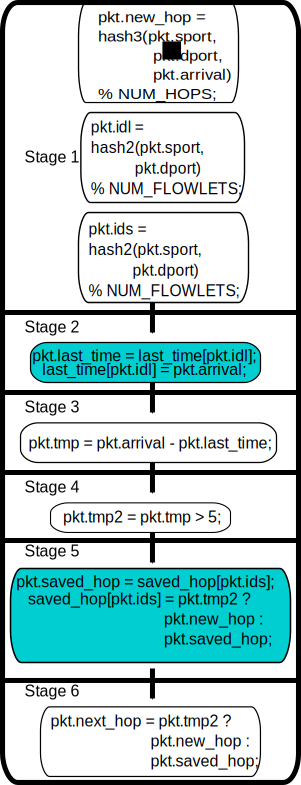
\includegraphics[width=0.8\columnwidth]{pipe.pdf}
\caption{Compiled 6-stage \absmachine pipeline implementing flowlet
switching.  Control flows from top to bottom. Atoms manipulating state are
shaded in blue.}
\label{fig:flowlet_pipeline}
\end{minipage}
\end{figure*}

We now illustrate programming using packet transactions in \pktlanguage, using
flowlet switching~\cite{flowlets} as an example. Flowlet switching is a
load-balancing algorithm that sends bursts of packets (called flowlets) from a
TCP flow on different paths, provided the bursts are separated by a large
enough time interval to ensure packets do not arrive out of order at a TCP
receiver. Figure~\ref{fig:flowlet_code} shows flowlet switching in
\pktlanguage. For simplicity, we hash only the source and destination ports; it
is easy to extend it to the full 5-tuple.

This example demonstrates the core language constructs in \pktlanguage. All
packet processing happens in the context of a packet transaction (the function
\texttt{flowlet} starting at line 17). The function's argument {\tt pkt}
declares the fields in a packet (lines 5--12)\footnote{We use fields to refer
to both packet headers such as source port ({\tt sport}) and destination port
({\tt dport}) and packet metadata ({\tt id}).} that can be referenced by the
function body (lines 18--32).  The function body can also modify persistent
switch state using global variables (e.g.  \texttt{last\_time} and
\texttt{saved\_hop} on lines 14 and 15, respectively).

Conceptually, the switch invokes the packet transaction function on each
incoming packet sequentially. To the programmer, the function modifies the
passed-in packet argument and runs to completion before processing the next
packet.  The function may invoke \textit{intrinsics} such as \texttt{hash2} on
line 23 to use hardware accelerators such as hash generators.  The \pktlanguage
compiler uses an intrinsic's signature to infer dependencies and supplies a
canned run-time implementation, but otherwise does not analyze an intrinsics's
internal behavior.

\subsection{Constraints on the language}
%%\pktlanguage relative to software
%%routers like Click~\cite{click} with greater flexibility and variable
%%performance.

The overall language is a constrained subset of C
(Table~\ref{tab:restrict}).  These constraints are required for
deterministic performance.  Memory allocation, unbounded iteration
counts, and unstructured control flow all cause variable performance,
which may prevent an algorithm from achieving line rate.
Furthermore, all accesses to a given array within one execution of a
transaction, i.e. one packet, must use the same array index. For
example, all read and write accesses to the array \texttt{last\_time}
use the index \texttt{pkt.id}, which is constant for each packet, but
can change between packets. This restriction mirrors restrictions on
memories, where supporting distinct read and write addresses every
clock cycle is challenging.\MA{Do we model this restriction in PISA?
  It would be better to add it to Sec 2.}

\begin{table}
  \begin{tabular}{p{0.9\columnwidth}}
    No iteration (while, for, do-while).\\
    No goto, break, or continue.\\
    No pointers.\\
    No dynamic memory allocation / heap.\\
    Array index is constant for each transaction execution.\\
    No access to data i.e. unparsed portion of the packet.\\
    No arrays in packet fields.\\
  \end{tabular}
  \caption{Restrictions in \pktlanguage}
  \label{tab:restrict}
\end{table}

\subsection{All-or-nothing compilation}

When compiled to a \absmachine machine (\S\ref{s:absmachine}), the
\pktlanguage compiler (\S\ref{s:compiler}) converts the code in
Figure~\ref{fig:flowlet_code} into the atom pipeline in
Figure~\ref{fig:flowlet_pipeline}. If it succeeds, the compiler
guarantees that the program will run at line rate on the target.
Otherwise, the compiler rejects the program outright; there is no
smooth tradeoff between a program's performance and its complexity.
This {\em all-or-nothing} compilation model is unusual for someone
programming other computational substrates such as a CPU, GPU, or
DSP. But, it reflects how routers and switches are used today. Routers
are rated for a particular line rate, regardless of the feature set
that an operator enables. 

% This all-or-nothing model provides
% predictable performance for free---in contrast to software-routers
% that need explicit support for it~\cite{dobrescu2012, wenfei15}.
% MA: I would just get rid of this last sentence. It's not really
% "free", you lose some capability.

\subsection{Limitations of packet transactions}

Packet transactions are a good fit for data-plane algorithms that do a
small amount of work per packet (i.e. where the amount of work can be
bounded at compile time) and manipulate only packet
headers. Data-plane algorithms like deep packet inspection and wan
optimization access packet payloads. These algorithms require a switch
to parse the packet payload as well---effectively parsing a huge
header consisting of each byte in the packet payload. Parsing deep
parse graphs is challenging at line rates of 1 GHz.\MA{So this is more
  a limitation of the parser than the transactional model. A better
  example might be an algorithm that manipulates a large amount of
  state, but does not need to run on every packet. For example,
  periodically scanning a list of numbers to find their average might
  be possible in hardware.}  Consequently, the limitations of packet
transactions merely reflect fundamental limitations of the underlying
hardware.
%% TODO: Move the parsing limitation into section 2 as a limitation of the machine itself,
%% not the packet transaction model itself.

%% TODO: Think of things in the middle between packet transactions and
%% the control plane. Trigger packets once in a while to do some clean
%% up operations, every so often. Explain that as a limitation of the
%% packet transaction model.

%% Move both of these things to section 2.
%% Instead of having 2.5, merge resource limits into 2.4 and create a new
%% subsection called limitations of line-rate switches.

%% Call 2.4 "limitations on the PISA model".
%% The focus is on algorithms that run at line rate and process a packet every clock cycle.
%% This poses restrictions.

%% Merge 2.4 and 2.5
%% Make a section that says: "What can PISA not do?" at the end of pisa.tex and add the two
%% limitations from line-rate: parsing and middle-plane computations.

\section{The \pktlanguage compiler}
\label{s:compiler}

% TODO: Add high-level diagram describing the compiler.
% for every pass, describe what it is, provide an example, show how it's much
% simpler than usual, and show what invariant it guarantees.
We now describe the \pktlanguage compiler frontend. The compiler frontend
operates only on sequential code blocks, allowing us to borrow well-established
techniques from the compiler literature~\cite{muchnik}. However, as we show
throughout this section, constraining \pktlanguage allows us to considerably
simplify the compiler relative to mainstream compilers.

\subsection{Lexing, parsing, and semantic analysis}
\pktlanguage's syntax is a subset of C, implying that all \pktlanguage are
well-formed C programs that can be compiled by a C compiler like
clang~\cite{clang}. We use clang's library interface~\cite{libclang} to
generate an Abstract Syntax Tree (AST) for a packet transaction written in
\pktlanguage. The remaining compiler passes all operate on an AST produced by
clang.

Embedding \pktlanguage within C has several benefits. It allows to reuse
clang's industrial strength frontend and catches several compiler errors with
no additional effort.  It also allows us to use C's macro preprocessor for
constants. Finally, opaque functions representing hardware primitives (e.g.
hashes and checksum), can be implemented using arbitrary C code and linked with
\pktlanguage code before running the resulting binary on our abstract machine.

\subsection{Converting to straight-line code}
A packet transaction's body can contain if-else statements that alter the
control flow of the program and complicate dependence analysis. We eliminate
if-else statements by transforming them into the C conditional operator,
starting from the innermost if statements and recursing outwards
(Figure~\ref{fig:if_convert}). This is similar to if
conversion~\cite{allen_if_conversion}, but is much simpler because only the if
and else constructs alter control flow in \pktlanguage and all other forms of
control transfers (break, continue, loops) are forbidden.
\begin{figure}
\begin{tiny}
\begin{lstlisting}
if (pkt.arrival_time - last_time[pkt.id1] > FLOWLET_THRESHOLD) {
  saved_hop[pkt.id0] = pkt.new_hop;
}
\end{lstlisting}
\end{tiny}
\begin{center}
is transformed into
\end{center}
\begin{tiny}
\begin{lstlisting}
pkt.tmp0 = pkt.arrival_time - last_time[pkt.id1] > FLOWLET_THRESHOLD;
saved_hop[pkt.id0] = pkt.tmp0 ? pkt.new_hop : saved_hop[pkt.id0];
\end{lstlisting}
\end{tiny}
\caption{Conversion to straight-line code}
\label{fig:if_convert}
\end{figure}

This transformation creates straight-line code, where control always passes
from one statement to the next without any branching. Straight-line code
considerably simplifies the rest of the compiler.

\subsection{Identifying state variables}

We next identify all state variables used in a packet transaction, both arrays
and scalars. State variables represent persistent state stored on the switch
that modifies the behavior of the packet transaction from one step to the next.
In Figure~\ref{fig:flowlet}, \texttt{last\_time} and \texttt{saved\_hop} are
both array-based state variables.

%%We handle state variables differently from packet variables for two reasons.
%%All operations on a particular state variable must happen within one
%%\absmachine atom. This reflects the reality that sharing state variables across
%%atoms or stages is technically challenging because it would require
%%multi-ported memories. Further, all state updates on a state variable should be
%%completed before the next packet is processed. Otherwise, the next packet could
%%see stale values, which would violate the transactional specification.

To identify state variables, we scan the straight-line AST produced by the
previous pass, looking for scalar variables or arrays. For each state variable,
we create a \textit{read flank} to read the state variable into a packet
temporary. For an array, we move the indexing expression into the prologue as
well making use of the fact that the array index remains constant for each
packet for all valid \pktlanguage programs. Next, we replace all occurences of
the state variable with the packet temporary, and create a \textit{write flank}
that writes the packet temporary back into the state variable.  Figure
~\ref{fig:stateful_flanks} illustrates this transformation on a fragment.

\begin{figure}
\begin{tiny}
\begin{lstlisting}
pkt.id1 = hash2(pkt.sport, pkt.dport) % 8000;
last_time[pkt.id1] = pkt.arrival_time;
\end{lstlisting}
\end{tiny}
\begin{center}
is transformed into
\end{center}
\begin{tiny}
\begin{lstlisting}
// Read prologue for last_time
pkt.id1 = hash2(pkt.sport, pkt.dport) % 8000;
pkt.last_time0 = last_time[pkt.id1];

pkt.last_time0 = pkt.arrival_time;

// Write epilogue for saved_hop and last_time
last_time[pkt.id1] = pkt.last_time0;
\end{lstlisting}
\end{tiny}
\caption{Adding read and write flanks for state variables}
\label{fig:stateful_flanks}
\end{figure}

At the end of this pass, the code resembles assembly code for a load-store
architecture: state variables are only accessed through reads and writes, and
all arithemtic operations happens on packet variables. Restricting the set of
operations on state variables allows us to simplify reasoning about state
variables when we compile \pktlanguage to the abstract machine
(\S\ref{s:machine}).

% Any reason, we should be running SSA after stateful_flanks and not the
% other way around? Run it and see.
% I tried this in jayhawk and things don't work. Here's why.
% Stateful_flanks almost always destroys SSA because if you have something any
% state variable write of the form s = pkt.f; it will be transformed into
% pkt.tmp = s;
% pkt.tmp = pkt.f;
% s = pkt.tmp;
% which already destroys SSA.

\subsection{Static Single-Assignment Form}
We next transform the code block within the packet transaction into static
single-assignment form (SSA)~\cite{ferrante_ssa}, a well-known intermediate
form used by many compilers where every variable is assigned exactly once.
While computing the SSA in general requires the use of clever graph
algorithms~\cite{post_dominators}, computing the SSA for \pktlanguage is
trivial because the code is in straight-line form by the time SSA is run.

To compute the SSA, we replace every definition of a packet variable with a new
packet variable and propagate this new packet variable until the next
definition of the same variable. State variables are already in SSA form
because after the state flanks have been added, every state variable is read
and written exactly once.

SSA simplifies further analysis. Because every variable is assigned exactly
once, there are no Write-After-Read or Write-After-Write dependencies; only
Read-After-Write dependencies remain. This, in turn, facilitates compilation
(\S\ref{s:absmachine}) to the backend.
\begin{figure}
\begin{tiny}
\begin{lstlisting}
pkt.id1 = hash2(pkt.sport, pkt.dport) \% 8000;
pkt.last_time0 = last_time[pkt.id1];
pkt.last_time0 = pkt.arrival_time;
last_time[pkt.id1] = pkt.last_time0;
\end{lstlisting}
\end{tiny}
\begin{center}
is transformed into
\end{center}
\begin{tiny}
\begin{lstlisting}
pkt.id10 = hash2(pkt.sport, pkt.dport) \% 8000;
pkt.last_time00 = last_time[pkt.id10];
pkt.last_time01 = pkt.arrival_time;
last_time[pkt.id10] = pkt.last_time01;
\end{lstlisting}
\end{tiny}
\caption{SSA transformation}
\label{fig:stateful_flanks}
\end{figure}

\subsection{Three-address code}
We next convert code into three-address code, where all
instructions are either reads / writes into stateful variables or carry out
packet manipulations of the form: \texttt{pkt.f1 = pkt.f2 op pkt.f3;} where
\texttt{op} includes all arithmetic, logical, and relational operators. We also
allow either pkt.f2 or pkt.f3 to be an opaque function call of multiple packet
fields, because \pktlanguage assumes opaque functions are supported in
hardware. Three-address code instructions are similar to P4's action primitives
~\cite{p4spec} and map one-to-one with RMT~\cite{rmt}'s VLIW instruction set.

To generate three-address code, we flatten expressions that are not
already legal three-address code, by introducing enough temporaries. For
instance, \texttt{pkt.f = pkt.f1 + pkt.f2 - pkt.f3;} would be flattened to
\texttt{pkt.tmp = pkt.f2 - pkt.f3;} followed by \texttt{pkt.f = pkt.f1 +
pkt.tmp;}

\begin{figure}[!h]
\begin{tiny}
\begin{lstlisting}
pkt.id00 = hash2(pkt.sport, pkt.dport) % 8000;
pkt.saved_hop00 = saved_hop[pkt.id00];
pkt.id10 = hash2(pkt.sport, pkt.dport) % 8000;
pkt.last_time00 = last_time[pkt.id10];
pkt.new_hop0 = hash3(pkt.sport, pkt.dport, pkt.arrival_time) % 64;
pkt.tmp1 = pkt.arrival_time - pkt.last_time00;
pkt.tmp00 = pkt.tmp1 > 5;
pkt.saved_hop01 = (pkt.tmp00) ? (pkt.new_hop0) : pkt.saved_hop00;
pkt.last_time01 = pkt.arrival_time;
pkt.next_hop0 = (pkt.tmp00) ? (pkt.new_hop0) : pkt.saved_hop00;
saved_hop[pkt.id00] = (pkt.tmp00) ? (pkt.new_hop0) : pkt.saved_hop00;
last_time[pkt.id10] = pkt.arrival_time;
\end{lstlisting}
\end{tiny}
\caption{Flowlet switching in three-address code}
\label{fig:three_address}
\end{figure}

\subsection{Code partitioning}
At this point, the code is still in sequential form. Code partitioning
turns sequential code into an atom grid that can be run by \absmachine , by
exploiting parallelism within and across pipeline stages.
To partition code, we carry out the following steps:
\begin{enumerate}
  \item Create a node for each statement in the packet transaction after
    expression flattening.
  \item Create a bidrectional edge between N1 and N2 where N1 is a read from a
    state scalar / state array and N2 is a write into the same state scalar /
    state array. This step captures the constraint that state is internal to an
    atom in \absmachine.
  \item Create an edge (N1, N2) for every pair of nodes N1, N2 where N2 reads
    a variable written by N1. This is the only dependency we need to check because
    control dependencies turn into data dependencies when generating straight-line
    code. Further, the use of SSA removes all write-after-read and write-after-write
    dependencies.
  \item Generate strongly connected components (SCCs) of the resulting graph
    (Figure~\ref{fig:deps}) and condense the SCCs to to create a directed
    acyclic graph (DAG) (Figure~\ref{fig:dag}). This step captures the
    constraint that all updates to state variables must reside within the same
    atom.
  \item Schedule the resulting DAG using critical path
    scheduling~\cite{crit_path_sched}, creating a new pipeline stage everytime
    one operation needs to follow another (Figure~\ref{fig:pipeline}).
\end{enumerate}

\begin{figure*}
  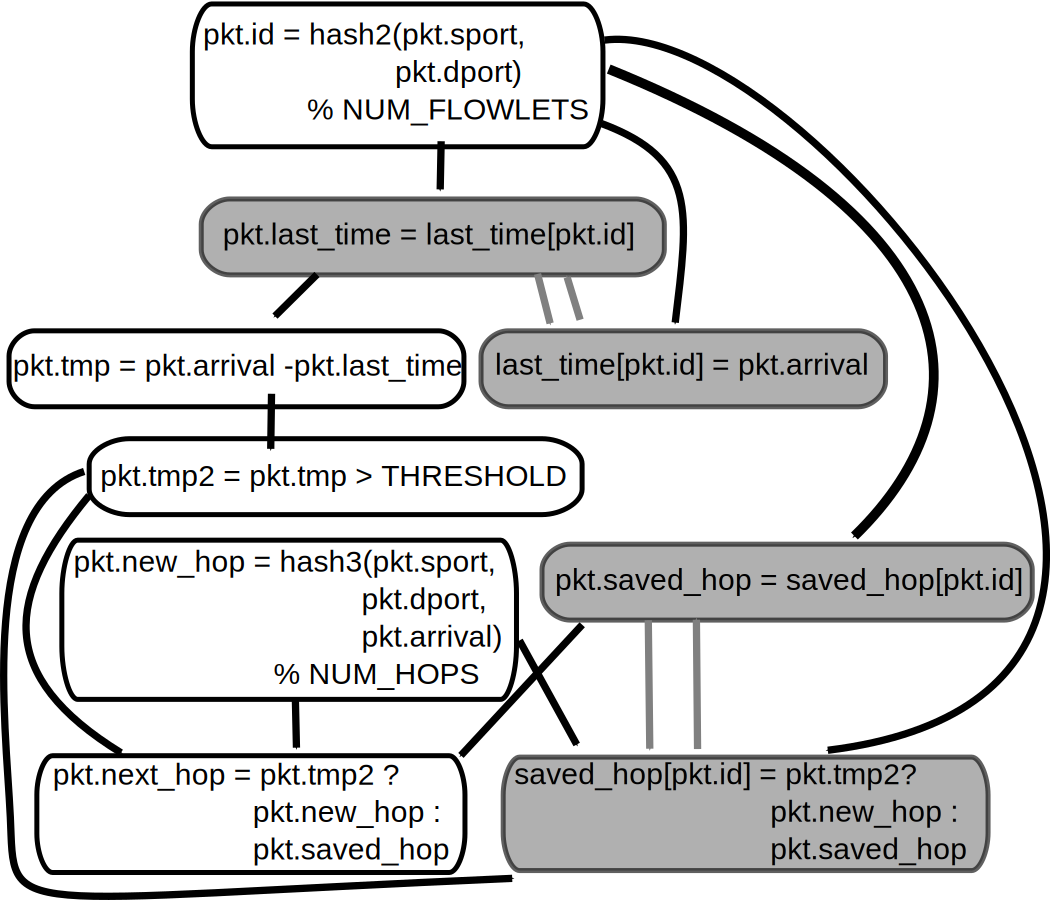
\includegraphics[width=\textwidth]{deps.pdf}
  \caption{Dependency graph of code shown in Figure~\ref{fig:three_address}}
  \label{fig:deps}
\end{figure*}

At this point, each strongly connected component can be turned into an atom for
\absmachine and the resulting pipeline implements the packet transaction.
Further, the atoms have a very stylized form. Stateless atoms contain exactly
one three-operand code instruction. Atoms that manipulate state contain at
least two statements: a read from a state variable and a write to a state
variable and optionally consist of one or more updates to the state variable.

\subsection{Constraints on atoms}
\label{ss:complexity}
So far, we haven't constrained the code in atom bodies in any way to reflect
hardware constraints. Expression flattening generates stateless atoms that each
have only one instruction. Further, because these instructions are in
three-operand code form, they map directly to the VLIW capabilities of
programmable switches.

Atoms that manipulate state can, in general, have multi-line atom bodies and it
is unclear whether these can be implemented at all. For instance, the update to
the state variable \texttt{saved\_hop} requires a read, followed by a
conditional update, followed by a write back. This section develops a general
technique to determine the implementability of stateful atoms, given
constraints on stateful atom bodies imposed by the hardware.

We first observe that constraints on stateful atoms can be written as program
sketches~\cite{bitstreaming, finite, sketch_manual}: a code fragment with fixed
and configurable parts. For instance, an atom with the constraint that it can
execute at most one programmable modify operation between a read and a write
operation to a stateful variable x can be represented as:
\begin{figure}
\begin{tiny}
\begin{lstlisting}
pkt.tmp = x;
pkt.tmp2 = pkt.tmp ?? (??);
x = pkt.tmp;
\end{lstlisting}
\end{tiny}
\caption{Sketch for single update operation to a state variable}
\label{fig:sketch_for_state}
\end{figure}
Here, the double question mark \texttt{??} stands for a
\textit{hole}~\cite{sketch_manual}. The hole is a placeholder for values from a
finite set that can be substituted in place of the hole. An automated program
synthesis~\cite{synthesis} tool called Sketch~\cite{sketch_manual} then
\textit{fills in} these holes to make the sketch equal to a specification.

As an example, if we want to implement the specification \texttt{x = x + 1;}
using the sketch in Figure~\ref{fig:sketch_for_state}, the Sketch tool would
fill the first hole with the value '+' from the finite set ('+', '-', '/', '*')
and the second hole with the value 1 from a finite set of integers specified as
input to the tool.

For the interested reader, a more detailed explanation of how Sketch works is
available in the appendix. For the purposes of the \pktlanguage compiler
though, we treat Sketch as a blackbox. We express the underlying constraints on
atoms as sketches, feed Sketch with an atom specification that needs to be
satisfied.  If there is a way to complete the sketch to satisfy the atom
specification, Sketch will find it, otherwise, it will determine that the
specification is unsatisfiable. For instance, the specification: \texttt{x = x
* x;} is unsatisfiable given the constraints in
Figure~\ref{fig:sketch_for_state}.

Using sketches to model constraints on atoms allows us to express constraints
very generically. At its core, a sketch is an incomplete imperative program,
and hence can express a variety of atom constaints. To show its generality, we
conside two such constraints in our evaluations: an in-order sequential CPU
that can execute exactly $N$ three-operand instructions and a combinatorial
circuit with a very specific form.

\begin{figure}
  \includegraphics[width=\columnwidth]{dag.pdf}
  \caption{DAG formed by condensing SCCs in Figure~\ref{fig:deps}}
  \label{fig:dag}
\end{figure}

%TODO: Maybe once we have enough examples of optimizations, we can roll those
%into SSA as saying how SSA makes it trivial to apply those optimizations.
% Again, this is compiler 101 for anyone who knows it.

\subsection{\tester: verifying compilations}

To conclude our description of the compiler, we describe our testing
infrastructure to verify that the compilation is correct i.e. the externally
visible behavior of the packet transaction (Figure~\ref{fig:flowlet}) is
indistinguishable from its pipelined implementation
(Figure~\ref{fig:pipeline}).

We verify correctness by feeding in the same set of test packets to both the
packet transaction and its implementation and comparing the outputs from both
programs on the set of externally visible fields. To create test packets, we
scan the packet transaction and generate the set of all packet fields read from
or written to by the transaction. We then initialize each of these fields by
sampling uniformly from the space of all 32-bit signed integers. In the future,
we plan to allow the user to specify more precise ranges for each packet field
that can be used for more directed testing.

To compare outputs from the packet transaction and its implementation, we track
renames that occur because of SSA. We compare each output field in the
transactional form with the last rename of the same output field in the
implementation. We then feed the same number of test packets to both the
specification and implementation and compare outputs at the end of the
pipeline. This allows to quickly ``spot check'' our compilations and was
instrumental in uncovering a few bugs in various compilation passes during
development.

\section{Evaluation}
\label{s:eval}

\begin{table*}[!t]
  \begin{scriptsize}
  \begin{tabular}{|p{0.15\textwidth}|p{0.8\textwidth}|}
  \hline
  Atom template & SKETCH shorthand\\
  \hline
  Write &
  {\begin{lstlisting}[style=customctable]
  x = mux2(pkt.f, ??);
  \end{lstlisting}} \\
  \hline
  Increment &
  {\begin{lstlisting}[style=customctable]
  x = mux3(x, pkt.f, ??) + mux2(1, 0);
  \end{lstlisting}} \\
  \hline
  ReadAddWrite &
  {\begin{lstlisting}[style=customctable]
  x = mux3(x, pkt.f, ??) + mux2(??, pkt.f);
  \end{lstlisting}} \\
  \hline
  \pbox{0.15\textwidth}
  {Predicated\\
  ReadAddWrite} &
  {\begin{lstlisting}[style=customctable]
  if(mux2(x, ??) rel_op mux3(pkt.f1, pkt.f2, ??)) {
    x = mux4(x, pkt.f1, pkt.f2, ??) + mux3(??, pkt.f1, pkt.f2);
  }
  \end{lstlisting}} \\
  \hline
  \pbox{0.15\textwidth}
  {If-Else\\
   ReadAddWrite} &
  {\begin{lstlisting}[style=customctable]
  if(mux2(x, ??) rel_op mux3(pkt.f1, pkt.f2, ??)) {
    x = mux4(x, pkt.f1, pkt.f2, ??) + mux3(??, pkt.f1, pkt.f2);
  } else {
    x = mux4(x, pkt.f1, pkt.f2, ??) + mux3(??, pkt.f1, pkt.f2)};
  }
  \end{lstlisting}} \\
  \hline
  Paired Updates &
  {\begin{lstlisting}[style=customctable]
  bit pred1 = mux3(x, y,  ??) rel_op mux3(pkt.f1, pkt.f2, ??);
  bit pred2 = mux3(x, y,  ??) rel_op mux3(pkt.f1, pkt.f2, ??);
  if (pred1) {
    x = mux4(x, pkt.f1, pkt.f2, ??) + mux3(??, pkt.f1, pkt.f2);
    y = mux4(y, pkt.f1, pkt.f2, ??) + mux3(??, pkt.f1, pkt.f2);
  } else if (pred2) {
    x = mux4(x, pkt.f1, pkt.f2, ??) + mux3(??, pkt.f1, pkt.f2);
    y = mux4(y, pkt.f1, pkt.f2, ??) + mux3(??, pkt.f1, pkt.f2);
  }
  \end{lstlisting}} \\
  \hline
  \end{tabular}
\end{scriptsize}
  \caption{Atom templates used in evaluation. rel\_op $\in \{<, >, != , ==\}$ stands for a relational operator. ?? refers to a SKETCH hole that can be filled in with an unsigned integer in the range $[0, 2^n]$.}
  \label{tab:templates}
\end{table*}

\begin{table*}[!t]
\begin{tabular}{|p{0.20\textwidth}|p{0.74\textwidth}|}
\hline
Algorithm & Stateful computation \\
\hline
Learning bloom filter & \pbox{0.74\textwidth}{Set membership bit on every packet.
                                              We ``learn'' a new packet by adding it to the set.}\\
\hline
%TODO: Ask Lavanya exactly how heavy hitters works.
Heavy Hitters~\cite{opensketch} & Increment Count-Min Sketch~\cite{cormode} on every packet \\
\hline
Flowlet switching~\cite{flowlets} & Update saved next hop if flowlet threshold is exceeded \\
\hline
RCP~\cite{rcp} & Accumulate RTT sum if RTT is under maximum allowable RTT \\
\hline
Periodic sampling & \pbox{0.74\textwidth}{Sample/Mark a packet if packet count reaches N; reset count at N.} \\
\hline
CONGA~\cite{conga} & \pbox{0.74\textwidth}{Update best path's utilization/id if we see a better path.\\
                                           Update best path utilization alone if it changes.} \\
\hline
\end{tabular}
\caption{Data-plane Algorithms}
\label{tab:algos}
\end{table*}

\begin{table*}[!t]
  \begin{tabular}{|p{0.20\textwidth}|p{0.04\textwidth}|p{0.09\textwidth}|p{0.14\textwidth}|p{0.14\textwidth}|p{0.14\textwidth}|p{0.05\textwidth}|}
  \hline
    & Write & Increment & ReadAddWrite & Predicated ReadAddWrite & IfElse ReadAddWrite & Paired Updates \\
  \hline
  Learning bloom filters & \cmark & \cmark & \cmark & \cmark & \cmark & \cmark \\
  \hline
  Heavy hitters          & \xmark & \cmark & \cmark & \cmark & \cmark & \cmark \\
  \hline
  Flowlet switching      & \xmark & \xmark & \xmark & \cmark & \cmark & \cmark \\
  \hline
  RCP                    & \xmark & \xmark & \xmark & \cmark & \cmark & \cmark \\
  \hline
  Periodic sampling & \xmark & \xmark & \xmark & \xmark & \cmark & \cmark \\
  \hline
  CONGA                  & \xmark & \xmark & \xmark & \xmark & \xmark & \cmark \\
  \hline
  \end{tabular}
\caption{Table summarizing algorithm implementability depending on the atoms provided by \absmachine}
\label{table:eval}
\end{table*}

%10. Alvin's feedback: Write about our experience writing these programs. Similar to Steven Chong's PLDI paper.
To evaluate \pktlanguage, we express several well-known data-plane algorithms
(Table~\ref{tab:algos}) using \pktlanguage and determine if they are
implementable on different \absmachine instances that differ in the stateful
atoms (Table~\ref{tab:templates}) that each provides.

\subsection{Experimental procedure}
As mentioned earlier, we consider only stateful atoms because we assume
three-address code instructions map one-to-one to stateless atoms for all
\absmachine instances. For simplicity, the stateful atoms we consider only
permit updates to state variables and forbid packet field updates that might be
mixed in with state updates. Assuming the \absmachine instance provides an atom
to read a state variable\footnote{We think this is reasonable because the
inability to read a state variable renders them meaningless!}, such packet
updates can be treated as stateless operations in subsequent pipeline stages.

To represent atoms succinctly using their atom templates in
Table~\ref{tab:templates}, we use a shorthand notation for SKETCH, using ``x''
and ``y'' for state variables, and using muxN(a1, a2, ..., aN) to represent a
configurable choice between N operands such as the choice made by the 2-to-1
multiplexer in Figure~\ref{fig:sketch}a.

Table~\ref{tab:templates} gradually increases the expressiveness of the
stateful atom provided by an \absmachine instance. These atoms form a
containment hierarchy: going from left to right in Table~\ref{table:eval}, each
atom is strictly more expressive than its predecessor to its left and hence can
express all algorithms that its predecessor can.

We now consider every atom from Table~\ref{tab:templates}, and every data-plane
algorithm from Table~\ref{tab:algos} to determine if each algorithm is
\textit{implementable} using a particular atom. We say an algorithm is
implementable using a particular atom if every stateful codelet within the
algorithm can be successfully mapped to that atom's template using the
procedure in \S\ref{ss:code_gen}.

\subsection{Interpreting these results}
Table~\ref{table:eval} presents our results. There are two ways to interpret
them. For a network programmer, the matrix in Table~\ref{table:eval} tells her
if a particular data-plane algorithm can be implemented at line rate after a
programmable switch has been built, assuming the \absmachine instance provides
a particular atom.

For an ASIC engineer designing programmable switching chips, the same table
describes the algorithms that are implementable with a particular atom. For
instance, the paired updates atom can implement all algorithms shown in
Table~\ref{table:eval}, while a simpler increment atom can implement only
two of the six algorithms.

These results will change as programmable switches evolve and network
programmers continuously push chip boundaries with new algorithms.  The larger
takeaway from this evaluation is that programming in \pktlanguage allows us to
rigorously determine if a particular high-level algorithm is implementable at
line rate using a particular atom and conversely, if a particular atom suffices
to implement a large number of algorithms.

\section{Related work}
\label{s:related}
NPUs: Tradeoffs are different here. Each stage can do very very little on a switch relative to an NPU. NPUs are Turing-complete; here, on a switch, programs either fit or don't. If they don't fit, you need to approximate.

P4 compiler (Lavanya's work): Complementary backend.

CMU work on pipelining datapaths: Verilog and circuits.

P4 itself: Too low level. NetASM: Once P4 needs an IR, NetASM might be a good choice.

Click: P4 paper wrote it off. We think its worth revisiting here.

Fastpass or Flexplane: Say that you love the abstraction they propose,
but would love to do it at higher line rates.

Click, Maple, Flexplane: Proposed transactions first. We are inspired by them.

%TODO: Flesh out the discussion section.
%1. designing atoms automatically from programs to move beyond the atom design process we used for this paper.
%2. weaker consistency semantics
%3. approximate semantics
%4. clarifying that the current compiler doesn't guarantee completeness,
%5. building an optimizing compiler
%6. handling multiple transactions

\section{Conclusion}
\label{s:conclusion}

This paper presented \pktlanguage, a C-like imperative language that allows
programmers to write packet-processing code using packet transactions:
sequential code blocks that are atomic and isolated from other such code
blocks. The \pktlanguage compiler compiles packet transactions to \absmachine,
a family of abstract machines based on programmable line-rate switch
architectures~\cite{flexpipe, xpliant, rmt}. Our results suggest that it is
possible to have both a familiar programming model and line-rate
performance---i.e. if the algorithm can indeed run at line rate.
Packet-processing languages are still in their infancy; we hope these results
prompt further work on programming abstractions for packet-processing hardware.

\section*{Acknowledgements}
We thank our shepherd, Bruce Maggs, the anonymous SIGCOMM reviewers, Amy
Ousterhout, and Pratiksha Thaker for their suggestions
that improved the presentation of the paper. This work was partly supported by
NSF grants CNS-1563826 and CNS-1563788. We thank the industrial partners of the
MIT Center for Wireless Networks and Mobile Computing (Wireless@MIT) for their
support.

\balance
{\small \bibliographystyle{abbrv}
\bibliography{paper}}

%% Atom, description, circuit, SKETCH
\appendix
\section{Atom templates and circuit diagrams for atoms}
The appendix provides circuit diagrams (Figures~\ref{fig:rw}--~\ref{fig:pairs})
and templates (Table~\ref{tab:atom_code}) for the atoms in
Table~\ref{tab:templates}. Table~\ref{tab:sketch_constructs} summarizes the
notation we use in this section.
\begin{table}[!htbp]
  \begin{minipage}{\columnwidth}
  \begin{scriptsize}
  \begin{tabular}{p{0.3\columnwidth}p{0.7\columnwidth}}
  Construct & Description \\
  \hline
  MuxN(a1, a2, \dots, aN) & \pbox{0.7\columnwidth}{N-to-1 multiplexer with enable bit.\\If enabled, return one of a1, a2, \dots aN.\\If disabled, return 0.}\\
  Opt(a)        & Return a or 0. (Equivalent to Mux1(a)). \\
  rel\_op(x, y) & Return one of $x < y$, $x > y$, $x != y$, $x == y$.\\
  Const() & Return an integer constant in the range [0, 31].\footnote{We restrict constants to 5 bits because all constants within stateful codelets in our dataplane algorithms are under 32. Larger ranges increase synthesis time.} \\
  x, y & State variables \\
  pkt\_1, pkt\_2 & Packet fields \\
  \end{tabular}
  \end{scriptsize}
  \caption{Notation used in atom templates}
  \label{tab:sketch_constructs}
\end{minipage}
\end{table}
\begin{table*}[!htbp]
\begin{scriptsize}
  \center
  \begin{tabular}{|p{0.09\textwidth}|p{0.73\textwidth}|p{0.04\textwidth}|}
      \hline
      Atom & Atom template & Element depth\\
\hline
\pbox{0.1\textwidth}{Write\\Figure~\ref{fig:rw}} &
{\begin{lstlisting}[style=customctable]
x = Mux2(pkt_1, Const());
\end{lstlisting}} &
1 \\

\hline
\pbox{0.1\textwidth}{ReadAddWrite\\(RAW)\\Figure~\ref{fig:raw}} &
{\begin{lstlisting}[style=customctable]
x = Opt(x) + Mux2(pkt_1, Const());
\end{lstlisting}} &
2 \\

\hline
\pbox{0.1\textwidth}
{Predicated\\
ReadAddWrite\\(PRAW)\\Figure~\ref{fig:praw}} &
{\begin{lstlisting}[style=customctable]
if (rel_op(Opt(x), Mux3(pkt_1, pkt_2, Const()))) {
  x = Opt(x) + Mux3(pkt_1, pkt_2, Const());
}
\end{lstlisting}} &
3 \\

\hline
\pbox{0.1\textwidth}
{If-Else\\
ReadAddWrite\\(IfElseRAW)\\Figure~\ref{fig:ifelseraw}} &
{\begin{lstlisting}[style=customctable]
if (rel_op(Opt(x), Mux3(pkt_1, pkt_2, Const()))) {
  x = Opt(x) + Mux3(pkt_1, pkt_2, Const());
} else {
  x = Opt(x) + Mux3(pkt_1, pkt_2, Const());
}
\end{lstlisting}} &
3 \\

\hline
\pbox{0.1\textwidth}
{Subtract (Sub)\\Figure~\ref{fig:sub}} &
{\begin{lstlisting}[style=customctable]
if (rel_op(Opt(x), Mux3(pkt_1, pkt_2, Const()))) {
  x = Opt(x) + Mux3(pkt_1, pkt_2, Const()) - Mux3(pkt_1, pkt_2, Const());
} else {
  x = Opt(x) + Mux3(pkt_1, pkt_2, Const()) - Mux3(pkt_1, pkt_2, Const());
}
\end{lstlisting}}&
4 \\

\hline
\pbox{0.1\textwidth}
{Nested Ifs\\(Nested)\\Figure~\ref{fig:nested}} &
{\begin{lstlisting}[style=customctable]
if (rel_op(Opt(x) + Mux2(pkt_1, pkt_2) - Mux2(pkt_1, pkt_2), Const())) {
 if (rel_op(Opt(x) + Mux2(pkt_1, pkt_2) - Mux2(pkt_1, pkt_2), Const())) {
  x = Opt(x) + Mux3(pkt_1, pkt_2, Const()) - Mux3(pkt_1, pkt_2, Const());
 } else {
  x = Opt(x) + Mux3(pkt_1, pkt_2, Const()) - Mux3(pkt_1, pkt_2, Const());
 }
} else {
 if (rel_op(Opt(x) + Mux2(pkt_1, pkt_2) - Mux2(pkt_1, pkt_2), Const())) {
  x = Opt(x) + Mux3(pkt_1, pkt_2, Const()) - Mux3(pkt_1, pkt_2, Const());
 } else {
  x = Opt(x) + Mux3(pkt_1, pkt_2, Const()) - Mux3(pkt_1, pkt_2, Const());
 }
}
\end{lstlisting}} &
6 \\

\hline
\pbox{0.1\textwidth}
{Paired Updates\\(Pairs)\\Figure~\ref{fig:pairs}} &
{\begin{lstlisting}[style=customctable]
if (rel_op(Mux2(x, y) + Mux2(pkt_1, pkt_2) - Mux2(pkt_1, pkt_2), Const())) {
 if (rel_op(Mux2(x, y) + Mux2(pkt_1, pkt_2) - Mux2(pkt_1, pkt_2), Const())) {
  x = Opt(x) + Mux3(pkt_1, pkt_2, Const()) - Mux3(pkt_1, pkt_2, Const());
  y = Opt(y) + Mux3(pkt_1, pkt_2, Const()) - Mux3(pkt_1, pkt_2, Const());
 } else {
  x = Opt(x) + Mux3(pkt_1, pkt_2, Const()) - Mux3(pkt_1, pkt_2, Const());
  y = Opt(y) + Mux3(pkt_1, pkt_2, Const()) - Mux3(pkt_1, pkt_2, Const());
 }
} else if (rel_op(Mux2(x, y) + Mux2(pkt_1, pkt_2) - Mux2(pkt_1, pkt_2), Const())) {
 if (rel_op(Mux2(x, y) + Mux2(pkt_1, pkt_2) - Mux2(pkt_1, pkt_2), Const())) {
  x = Opt(x) + Mux3(pkt_1, pkt_2, Const()) - Mux3(pkt_1, pkt_2, Const());
  y = Opt(y) + Mux3(pkt_1, pkt_2, Const()) - Mux3(pkt_1, pkt_2, Const());
 } else {
  x = Opt(x) + Mux3(pkt_1, pkt_2, Const()) - Mux3(pkt_1, pkt_2, Const());
  y = Opt(y) + Mux3(pkt_1, pkt_2, Const()) - Mux3(pkt_1, pkt_2, Const());
 }
}
\end{lstlisting}} &
6 \\
\hline

  \end{tabular}
  \end{scriptsize}
  \caption{SKETCH code for atoms described in Table~\ref{tab:templates}}
  \label{tab:atom_code}
\end{table*}


\newpage 
\begin{figure*}[!htbp]
  \center
  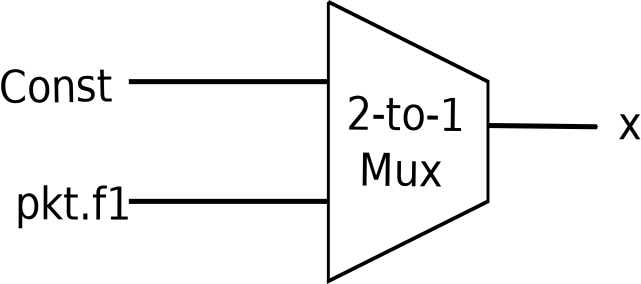
\includegraphics[width=\columnwidth]{rw.pdf}
  \caption{Circuit for Write atom with depth 1.}
  \label{fig:rw}
\end{figure*}
\begin{figure*}[!htbp]
  \center
  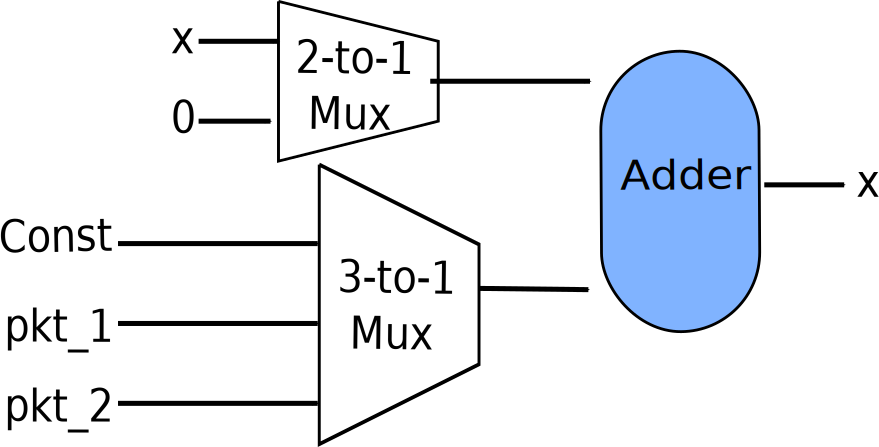
\includegraphics[width=\columnwidth]{raw.pdf}
  \caption{Circuit for RAW atom with depth 2.}
  \label{fig:raw}
\end{figure*}
\begin{figure*}[!htbp]
  \center
  \includegraphics[width=\columnwidth]{pred_raw.pdf}
  \caption{Circuit for PRAW atom with depth 3.}
  \label{fig:praw}
\end{figure*}
\newpage
\begin{figure*}[!htbp]
  \center
  \includegraphics[width=\columnwidth]{if_else.pdf}
  \caption{Circuit for IfElseRAW atom with depth 3.}
  \label{fig:ifelseraw}
\end{figure*}
\begin{figure*}[!htbp]
  \center
  \includegraphics[width=\columnwidth]{sub.pdf}
  \caption{Circuit for Sub atom with depth 4.}
  \label{fig:sub}
\end{figure*}

\newpage
\begin{figure*}[!htbp]
  \includegraphics[width=\textwidth]{nested.pdf}
  \caption{Circuit for Nested atom with depth 6.}
  \label{fig:nested}
\end{figure*}

\newpage
\begin{figure*}[!htbp]
  \includegraphics[width=0.95\textwidth]{pairs.pdf}
  \caption{One-half of the circuit for the Pairs atom with depth 6. The other
  half is identical, except that it updates y instead of x, and isn't shown for
simplicity. The shaded regions denote the differences in the Pairs atom
relative to the Nested atom: the predicates can depend on both x and y in the Pairs
atom.}
\label{fig:pairs}
\end{figure*}

\end{document}
